\documentclass[usenames,dvipsnames]{beamer}

%------------------------
% IMPORT PACKAGES
%-----------------------
\usepackage{graphicx}
\usepackage[dvipsnames]{xcolor}
\usepackage{amsthm}
\usepackage{amssymb}

\usepackage{booktabs}
\usepackage{dcolumn}
\usepackage{threeparttable}
\usepackage{adjustbox}
\usepackage{showframe}

\usepackage{mathtools}
\usepackage{tikz}
\usetikzlibrary{backgrounds,fit, positioning,shapes}
\usetikzlibrary{overlay-beamer-styles}
\usetikzlibrary{shapes.geometric, arrows,backgrounds,fit,positioning}
\usepackage{url}
\def\UrlBreaks{\do\/\do-}
\usepackage{caption}
\usepackage[absolute,overlay]{textpos}
\usepackage{fancyvrb}
\usepackage{array}

\newcommand{\source}[1]{\caption*{\tiny Adapted from: {#1}} }
\newcommand{\eqcolon}{\mathrel{\resizebox{\widthof{$\mathord{=}$}}{\height}{ $\!\!=\!\!\resizebox{1.2\width}{0.8\height}{\raisebox{0.23ex}{$\mathop{:}$}}\!\!$ }}}

\usetheme[sectionpage=none, progressbar=frametitle, numbering=fraction, titleformat=allcaps]{metropolis}

\titlegraphic{%
  \begin{picture}(0,0)
    \put(190,15){\makebox(0,0)[rt]{
\includegraphics[width=2.5cm]{Images/polimi_name_bn.png}}}
  \end{picture}}

\newtheorem{mydef}{\alert{Definition}}[section]

\AtBeginSection[]{
\begin{frame}{Talk Overview}
\tableofcontents[currentsection]
\end{frame}
\frame{\sectionpage}
}

\mode<presentation>
{
	\usetheme{metropolis}  
	\usecolortheme{default}
	\usefonttheme{default}  
	\useinnertheme{circles}
	\setbeamertemplate{navigation symbols}{}
	\setbeamertemplate{caption}[numbered]
	\setbeamerfont{caption}{size=\footnotesize}
	\setbeamerfont{bibliography entry author}{size=\footnotesize,series=\normalfont}
	\setbeamerfont{bibliography entry title}{size=\footnotesize,series=\bfseries}
	\setbeamerfont{bibliography entry location}{size=\footnotesize,series=\normalfont}
	\setbeamerfont{bibliography entry note}{size=\footnotesize,series=\normalfont}

} 

\addtobeamertemplate{navigation symbols}{}{%
	\usebeamerfont{footline}%
	\usebeamercolor[fg]{footline}%
	\hspace{1em}%
	%\insertframenumber/\inserttotalframenumber
}

\newcommand{\backupbegin}{
	\newcounter{framenumberappendix}
	\setcounter{framenumberappendix}{\value{framenumber}}
}
\newcommand{\backupend}{
	\addtocounter{framenumberappendix}{-\value{framenumber}}
	\addtocounter{framenumber}{\value{framenumberappendix}} 
}

\title{Blockchain Notarization: Extensions to the OpenTimestamps Protocol}
\author{\textbf{Andrea Brandoli} \qquad \qquad \qquad 
Supervisors: Daniele Marazzina,\\ \hspace*{6.78cm} Ferdinando M. Ametrano}
\date{16$^{\text{th}}$ April 2019}


\setbeamertemplate{bibliography entry title}{}
\setbeamertemplate{bibliography entry location}{}

\begin{document}

	\AtBeginSection[]{
	\begin{frame}[noframenumbering]{Outline}
		\small \tableofcontents[currentsection, hideothersubsections]
	\end{frame} 
	}

    \begin{frame}
        \titlepage
    \end{frame}
    
    \begin{frame}{Introduction}
        \begin{itemize}
            \item \alert{Notarization} of digital documents is traditionally achieved by a trusted certification authority.
            \item A notary public could be malevolent and represents a \alert{single point of failure}.
            \item An application built upon a \alert{distributed system} reaching consensus in a \alert{decentralized way} can greatly strengthen the notarization process.
            \item The Bitcoin blockchain, the most reliable decentralized system, can be used as a notary in a procedure called \alert{timestamping}.
            \item The open-source protocol \alert{OpenTimestamps} aims to be a standard for timestamping and solves a scalability issue.
        \end{itemize}
    \end{frame}
    
    \section{Distributed Consensus}
    \subsection{Distributed Systems}
    \begin{frame}{Distributed Systems}
       \begin{mydef}[distributed system]
       A distributed system is a system whose components are located on different networked computers, which communicate and coordinate their actions by passing messages to one another. The components interact with one another in order to achieve a common goal.
       \end{mydef}
       \alert{Examples}:
       \begin{itemize}
           \item ATM points.
           \item Computers in cloud.
           \item Modern smartphones.
       \end{itemize}
    \end{frame}
        
    \begin{frame}{Distributed Systems: Pros vs. Cons}
        \begin{minipage}[t]{0.5\linewidth}
        \noindent
        \alert{PROS:}
        \begin{itemize}
            \item Scalability.
            \item Performance.
            \item Fault tolerance.
            \item Reliability.
            \item Availability
        \end{itemize}
        \end{minipage}\hfill
        \begin{minipage}[t]{0.5\linewidth}
        \noindent
        \alert{CONS:}
        \begin{itemize}
            \item Security.
            \item Consensus.
        \end{itemize}
        \end{minipage}
        
        \bigskip
        Thus, the main challenge of distributed systems is to achieve \alert{distributed consensus} in the presence of a number of \alert{faulty processes}.
    \end{frame}
     
    \subsection{The Consensus Problem}  
    \begin{frame}{The Consensus Problem}
        \begin{itemize}
            \item Networks are composed by many agents, called \alert{nodes}.
            \item Nodes are either \alert{honest} or \alert{byzantine}.
            \item They could also be \alert{correct} and \alert{faulty}, but not as alternatives to honest and byzantine.
        \end{itemize}
        \begin{mydef}[consensus]
            There are $n$ nodes, of which at most $f$ might crash, i.e., at least $n-f$ nodes are correct. Node $i$ starts with a proposed value $v_{i}$. The nodes must decide for one of those values, satisfying the following properties:
            \begin{itemize}
                \item Agreement: All correct nodes decide for the same proposal.
                \item Termination: All correct nodes terminate in finite time.
                \item Validity: The decision value must be the proposal of some proposer.
            \end{itemize}
        \end{mydef}
    \end{frame}
        
    \begin{frame}{Byzantine Agreement in an asynchronous network}
           \begin{itemize}
               \item Is it possible to achieve \alert{distributed consensus} in an \alert{asynchronous} network in presence of \alert{byzantine} nodes ?
               \item The \alert{Byzantine General's Problem} is the abstraction of such situation.
           \end{itemize}
           More precisely:
           \begin{mydef}[byzantine general's problem]
            A commanding general must send an order to his $n-1$ lieutenant generals such that the following conditions are satisfied:
            \begin{itemize}
                \item All loyal lieutenants obey the same order.
                \item If the commanding general is loyal, then every loyal lieutenant obeys the order he sends.
            \end{itemize}
           \end{mydef}
	        
    \end{frame}
        
        \begin{frame}{Impossibility Result}
            
            \begin{itemize}
                \item Achieving \alert{distributed consensus} in an asynchronous network in presence of byzantine nodes is a very \alert{hard problem}.
                \item Fisher, Lynch and Paterson \cite{Fischer:1985:IDC:3149.214121} formally proved that it is \alert{impossible} to reach distributed consensus in an asynchronous network with \alert{one faulty process}, even for a \alert{binary} variable.
                \item So how Satoshi Nakamoto reaches consensus in \alert{Bitcoin}, a decentralized, distributed, peer-to-peer network ?
            \end{itemize}
            
        
            % \begin{itemize}
            % \item It is \alert{impossible} to reach distributed consensus in an asynchronous network with \alert{one faulty process}, even for a \alert{binary} variable.
        
            % \item A non-rigorous proof could be:
            % \end{itemize}
        
            % \begin{figure}
            % \centering
            % \begin{minipage}{.5\textwidth}
            % \centering
            % 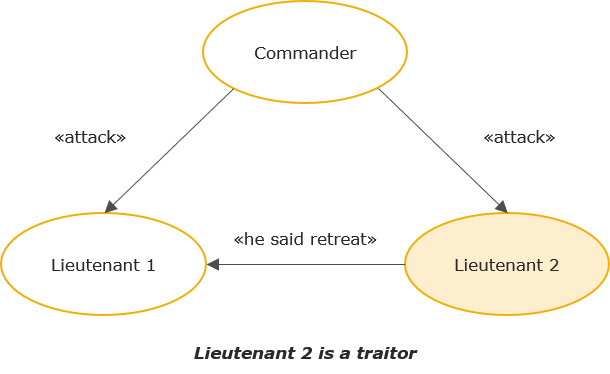
\includegraphics[width=0.8\linewidth]{Images/scenario1.png}
            % \caption{Lieutenant 2 is a traitor.}
            % \end{minipage}%
            % \begin{minipage}{.5\textwidth}
            % \centering
            % 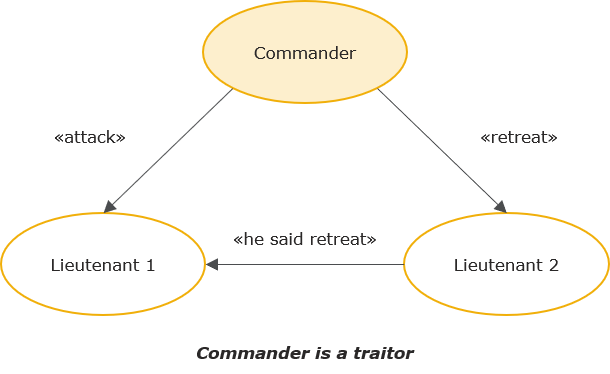
\includegraphics[width=0.8\linewidth]{Images/scenario2.png}
            % \caption{Commander is a traitor.}
            % \end{minipage}
            % \end{figure}
            
            % \begin{itemize}
            %     \item A \alert{formal} proof is made by Fisher, Lynch and Paterson.
            %     \item How Satoshi Nakamoto reaches consensus in \alert{Bitcoin} ?
            % \end{itemize}
            
        \end{frame}
    
    \section{Nakamoto Consensus in Bitcoin}
    \subsection{Eventual Consistency}
    
    \begin{frame}{Bitcoin as an Example of Eventual Consistency}
        \begin{itemize}
            \item \alert{Bitcoin} is a distributed, decentralized, peer-to-peer electronic payment system based on \alert{cryptographic proof}.
            \item The Bitcoin network is subjected to \alert{network partition}.
            \item It is inherently characterized by a trade-off between:
                \begin{itemize}
                    \item \alert{Consistency}: All nodes agree on the current state.
                    \item \alert{Availability}: The system is operational and instantly processing incoming requests.
                    \item \alert{Partition tolerance}: The ability to continue operating correctly even in the presence of a network partition.
                \end{itemize}
            \item CAP theorem proves that is \alert{impossible} to achieve \alert{simultaneously} the three properties.
            \item Nakamoto's intuition has been to relax the \alert{agreement} property in the consensus definition to hold \alert{probabilistically}, to reach \alert{eventual consistency}.
        \end{itemize}
    \end{frame}
    
    \subsection{Bitcoin Design}
    
    \begin{frame}{Double Spending Problem}
        \begin{itemize}
            \item In a digital cash scheme, a \alert{single digital token}, being just a file that can be duplicated, can be \alert{spent twice}. 
            \begin{figure}
            \centering
            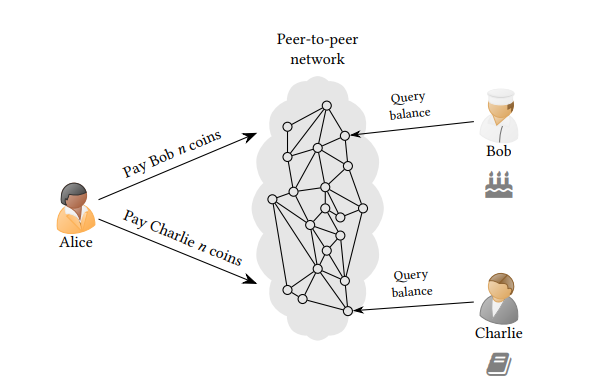
\includegraphics[keepaspectratio, height=0.5\textheight, width=0.5\textwidth]{Images/double-spending.png}
            \caption{Illustration of the double spending problem.}
            \end{figure}
            \item Nakamoto solves the \alert{double spending problem} combining \alert{cryptography} and \alert{social incentives}. But first, some protocol's mechanics.
            \end{itemize}
    \end{frame}
    \begin{frame}{Transactions in Bitcoin}
        \begin{itemize}
            \item A \alert{bitcoin} is defined as a chain of digital signatures.
            \item Coins cannot be combined, subdivided or transferred, but only \alert{entirely consumed} as transaction inputs (TxIn) to create new output coins (TxOut).
            \item A TxOut can be in two states: \alert{spent} or \alert{unspent}.
            \item The \alert{UTXO} is the set of current unspent transactions.
            \item A \alert{TxOut} consists of an amount of bitcoins and a \alert{locking script}, a cryptographic puzzle which determines the spending conditions.
            \item A \alert{TxIn} consists of a pointer referencing the UTXO that it consumes and an \alert{unlocking script}, the solution to solve the locking one.
        \end{itemize}
    \end{frame}
    
    \begin{frame}{The Blockchain}
        \begin{figure}
        \centering
        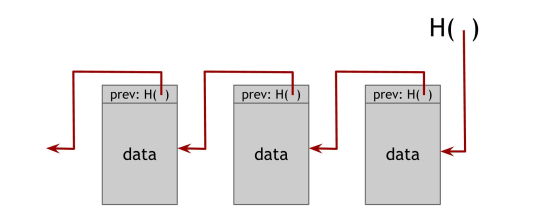
\includegraphics[width=0.7\linewidth]{Images/blockchain.png}
        \caption{Blockchain as a hash pointer linked list.}
        \end{figure}
        \begin{itemize}
            \item Transactions are recorded in a \alert{distributed ledger}, the \alert{blockchain}, formally a hash pointer linked list.
            \item The \alert{cryptographic link} between blocks requires computing power to be created.
            \item A block is \alert{valid} only if it includes valid transactions.
        \end{itemize} 
    \end{frame}

    \begin{frame}{Mining \& Proof of Work}
        \begin{itemize}
            \item All network nodes \alert{validate} and \alert{clear} all transactions.
            \item Special nodes, called \alert{miners}, compete to finalize a new block of transactions, providing \alert{proof-of-work}, which consists of finding a special number \alert{x} called \alert{nonce} s.t.
            $$\text{SHA256}(\text{SHA256}(\underbrace{... \| \text{prev\_block\_header\_hash} \| ... \| x}_{\text{Candidate Block Header}})) < \frac{2^{224}}{d}.$$
            \item The miner who \alert{first} find it is rewarded with the issuance of new bitcoins in a special \alert{coinbase} transaction.
            \item Miners solve the \alert{double spending problem}:
            \begin{itemize}
                \item A double spending transaction invalidates a block.
                \item The bitcoin reward would have removed.
                \item The winning miner would have wasted his work.
                \item Proof-of-work ensures \alert{blockchain immutability}.
            \end{itemize}
        \end{itemize}    
    \end{frame}
    
    \section{Blockchain Timestamping}
    \subsection{Notarization}
    \begin{frame}{Notarization}
    \begin{itemize}
        \item \alert{Notarization} is the official fraud-deterrend process that assures the parties of a transaction that a document is \alert{authentic} and can be \alert{trusted}.
        \item Traditionally, it is achieved by a trusted certification authority which represents a \alert{single point of failure}.
        \item Need to \alert{decentralize} the source of trust to be reliable even if the security of such central authority is violated, using the Bitcoin blockchain as a \alert{notary} for \alert{timestamping}.
        \end{itemize}
        \begin{mydef}[timestamp]
            A timestamp is a proof that some data $d$ existed prior to a certain time $t$ and in a certain state.
        \end{mydef}
    \end{frame}
    
    \subsection{Commitment Operations}
    \begin{frame}{Commitment Operations}
        \begin{itemize}
            \item To create a timestamp, data $d$ has to \alert{cause} an event that could not have been generated without the existence of $d$, must be \alert{attested} to time $t$ and can be \alert{publicly observed}.
            \item A \alert{good} timestamp must become \alert{invalid} even if a \alert{single bit} of the input data is modified.
            \item What is published on the blockchain is a \alert{commitment} to $d$.
            \end{itemize}
            \begin{mydef}[commitment operation]
            A function $C: X \rightarrow Y$ is a commitment operation if given $x_{1} \in X$ it is not feasible to compute $x_{2} \in X$ s.t. $x_{1} \neq x_{2}, C(x_{1}) = C(x_{2})$.
            \end{mydef}
            \alert{Examples}:
            \begin{itemize}
                \item append: \textquotedblleft hello\textquotedblright $\xrightarrow{\text{append(\textquotedblleft world\textquotedblright)}}$ \textquotedblleft helloworld\textquotedblright.
                \item prepend: \textquotedblleft world\textquotedblright $\xrightarrow{\text{prepend(\textquotedblleft hello\textquotedblright)}}$ \textquotedblleft helloworld\textquotedblright.
            \end{itemize}
    \end{frame}
    
    \begin{frame}{Hash Functions}
        \begin{itemize}
            \item However, both \textquotedblleft append\textquotedblright and \textquotedblleft prepend\textquotedblright commitment operations are \alert{not good} for timestamping:
            \begin{itemize}
                \item They do not \alert{hide} input data.
                \item Outputs are always \alert{bigger} in size.
            \end{itemize}
            \item \alert{Hash functions} map input data of \alert{arbitrary length} into hash values, i.e., outputs of \alert{fixed length}:
            \begin{itemize}
                \item \alert{Preimage resistant} (one-wayness): given $h(x)$ it is not feasible to compute $x$.
                \item \alert{Second-preimage resistant}: given $x$ it is not feasible to compute $y$ s.t. $x \neq y$, $h(x)=h(y)$.
                \item \alert{Collision resistant}: it is not feasible to find $x, y$ s.t. $x \neq y$, $h(x)=h(y)$.
            \end{itemize}
            \item An hash value represents a \alert{digital fingerprint}.
            \item Bitcoin uses \alert{SHA256}: outputs have a fixed size of 256-bit.
        \end{itemize}
    \end{frame}
    
    \subsection{Timestamping Procedure}
    \begin{frame}{Timestamping Procedure}
        \begin{itemize}
            \item A generic data file can be \alert{hashed} to produce a short unique identifier.
            \item Such a \alert{digital fingerprint} can be associated to a particular Bitcoin transaction, called \alert{null data transaction}.
            \item These transactions make use of \alert{OP\_RETURN}, an opcode script which allows to add up to 80 bytes of arbitrary data in a \alert{provably unspendable} transaction.
            \item Such transaction \alert{commits} to a specific field of the block header, called \alert{merkleroot}, which is the root of a binary tree that summarize all the transactions in a block.
            \item Blockchain \alert{immutability} provides \alert{timestamping}, proving the data file existance at that moment in time in that specific status.
        \end{itemize}    
    \end{frame}
    
    \section{OpenTimestamps}
    \subsection{OpenTimestamps Protocol}
    \begin{frame}{OpenTimestamps}
        \begin{itemize}
            \item Blockchain timestamping have some \alert{downsides}:
            \begin{itemize}
                \item Not efficient: it requires one transaction per document.
                \item Lack of standardization.
            \end{itemize}
            \item \alert{OpenTimestamps} is an open-source protocol that aims to be a \alert{standard} for blockchain timestamping.
            \item It defines a set of rules for \alert{conveniently} creating \alert{provable timestamps} and later \alert{independently verifying} them.
            \item A \alert{proof} made with OpenTimestamps consists in a list of \alert{commitment operations} applied in sequence to the document, ending with one or more \alert{time attestations}.
            \item It proposes a \alert{solution} to the \alert{scalability problem}.
        \end{itemize}
    \end{frame}
    
    \begin{frame}{OpenTimestamps as a Scalability Solution}
        \begin{itemize}
            \item OpenTimestamps allows to \alert{aggregate} up to an \alert{infinite number} of document in a single transaction.
            \item The trick is to compose documents in a \alert{merkle tree} and to timestamp only the \alert{root} of that tree.
        \end{itemize}
        \begin{figure}
        \centering
        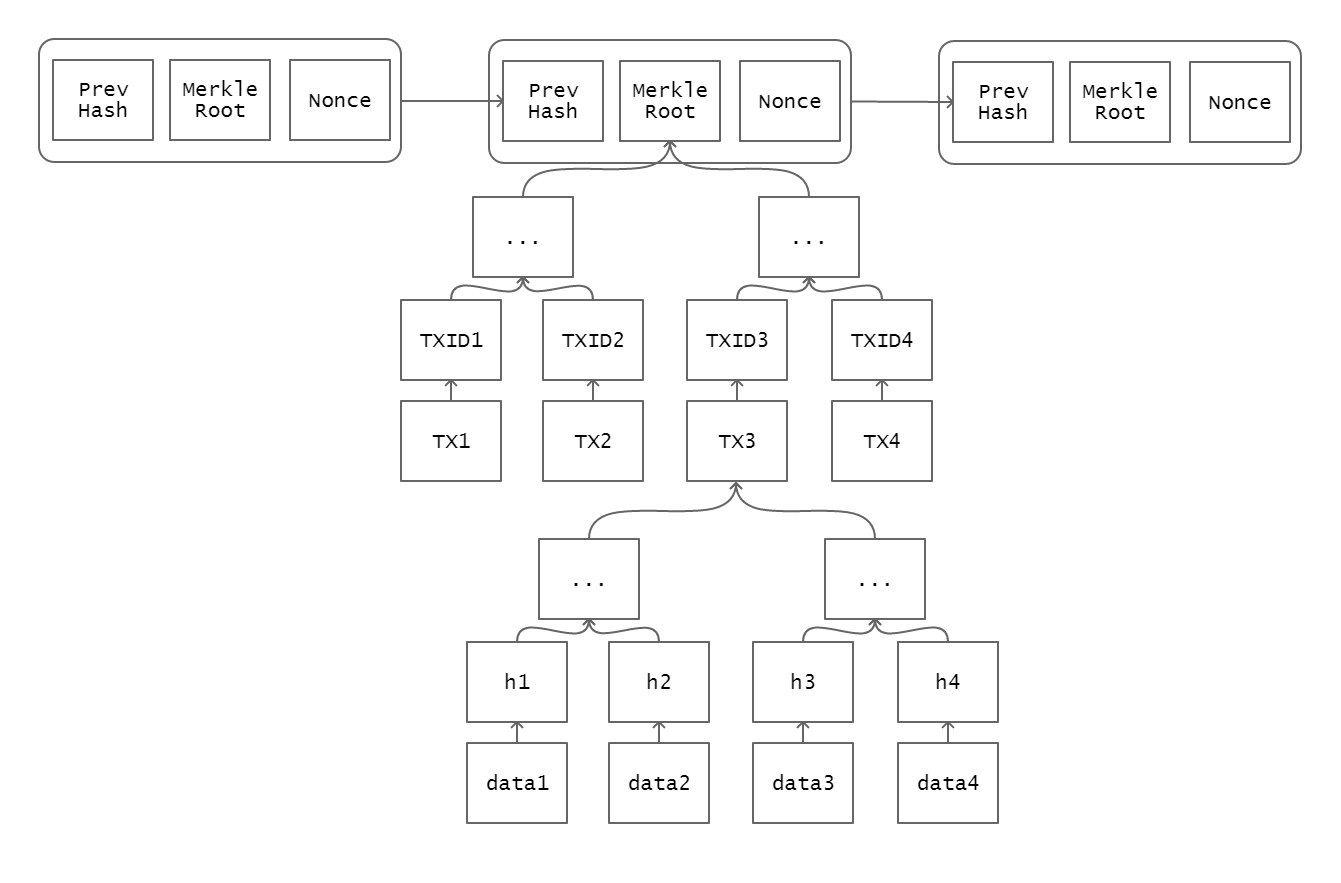
\includegraphics[width=0.6\linewidth]{Images/bitcoin-chain-calendar.png}
        \caption{OTS scalability solution.}
        \end{figure}
    \end{frame}
    
    \begin{frame}{OpenTimestamps as a Scalability Solution}
        \begin{itemize}
            \item Moreover, \alert{aggregation servers} collect hash values and periodically \alert{aggregate} them in a single merkle tree.
            \item Aggregation servers are \alert{efficient} but \alert{not convenient}: to obtain a proof you must wait for the transaction to be included in a block.
            \item To provide proofs almost \alert{instantly}, OpenTimestamps makes use of \alert{public calendar servers}.
            \item Aggregation servers submit the merkleroot to a calendar server, which \alert{promise} that every submitted digest will be timestamped with Bitcoin.
            \item Proofs made this way are \alert{incomplete}, but they can be \alert{upgraded} once the blockchain has completed the timestamp, \alert{adding} the path up the the \alert{block header}.
        \end{itemize}
    \end{frame}
    
    \subsection{A Practical Use Case}
    
    \begin{frame}{A Practical Use Case: Aim of the Project }
        \begin{itemize}
            \item The author, in partnership with \alert{DGI} (Digital Gold Institute) and \alert{ANIA} (Associazione Nazionale fra le Imprese Assicuratrici) worked on a \alert{practical use case} of blockchain timestamping.
            \item The aim of the project is to provide a fully operating \alert{timestamping service}.
            \item It is build upon OpenTimestamps, while marginally \alert{improving} and \alert{extending} such protocol with additional features.
            \item For example, any insurance company could make use of it to grant \alert{authenticity} of its associates policies.
            \item Simply, it could be useful whenever a \alert{digital signature} is involved.
        \end{itemize}
    \end{frame}
    
    \begin{frame}{Architecture of the solution}
        \begin{itemize}
            \item The \alert{architecture} of the solution consists of \alert{three cloud-servers}, accessible from outside via traditional network elements (DNS server, reverse proxy, firewall, etc.).
            \item Such elements transparently remap host names under the domain \textquotedblleft aniasafe.it\textquotedblright.
            \item The three servers are divided in a \alert{front-end} server and two \alert{back-end} servers:
            \begin{itemize}
                \item \alert{Front-end}: hosts the public \alert{web interface} (\url{https://timestamp.aniasafe.it}). 
                \item \alert{Back-end}: they both run a \alert{calendar server} connected to a local Bitcoin node: (\url{https://calendar.aniasafe.it}) for mainnet, (\url{https://test-calendar.aniasafe.it}) for testnet.
            \end{itemize}
        \end{itemize}
    \end{frame}
    
     \begin{frame}{Architecture of the solution}
     \begin{figure}
         \centering
         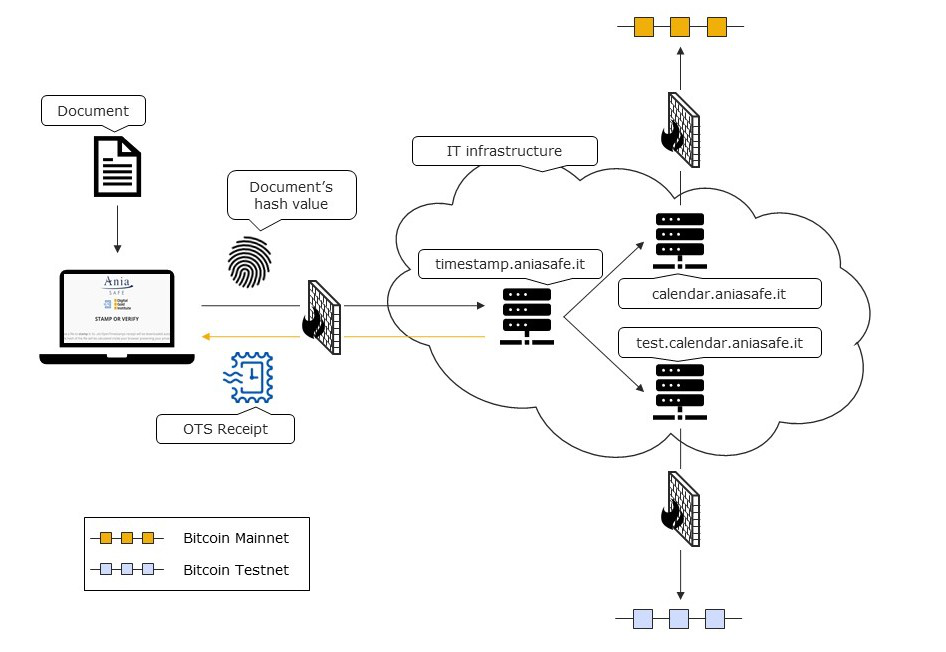
\includegraphics[width=0.92\linewidth]{Images/project-stamping.png}
         \caption{Architecture of the solution}
     \end{figure}
    \end{frame}
    
    \begin{frame}{Web Interface}
        \begin{itemize}
            \item The front-end server hosts the \alert{web interface}.
            \item The underlying \alert{JavaScript library} defines the \alert{main functions} invoked when a user interacts with the web interface: \textquotedblleft \alert{stamp}\textquotedblright, \textquotedblleft \alert{verifyTimestamp}\textquotedblright and \textquotedblleft \alert{upgradeTimestamp} \textquotedblright.
            \item The \alert{JS library} has been extended for \alert{additional features}:
            \begin{itemize}
                \item \alert{Testnet} as an alternative chain.
                \item \alert{Multi-validation}: the original protocol supports timestamping on multiple chains, but the verification of one attestation at a time.
                \item \alert{Esplora} (block-explorer): a new class has been created to query Esplora's API correctly.
            \end{itemize}
        \end{itemize}
    \end{frame}
    
     \begin{frame}{Web Interface: Stamping}
     \begin{figure}
         \centering
         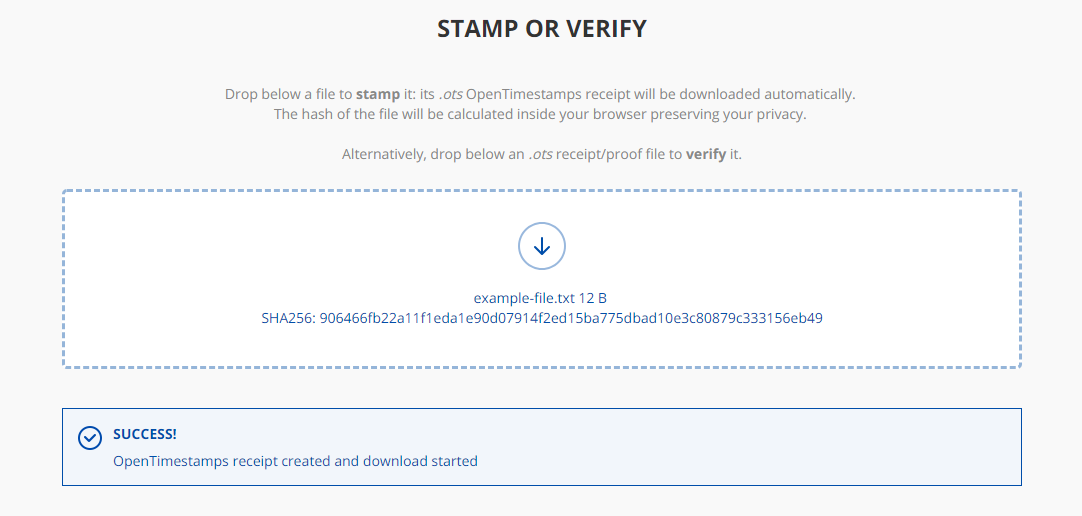
\includegraphics[width=1\linewidth]{Images/stamping.png}
         \caption{Stamping}
         
     \end{figure}
    \end{frame}
    
    \begin{frame}{Web Interface: Verifying}
     \begin{figure}
         \centering
         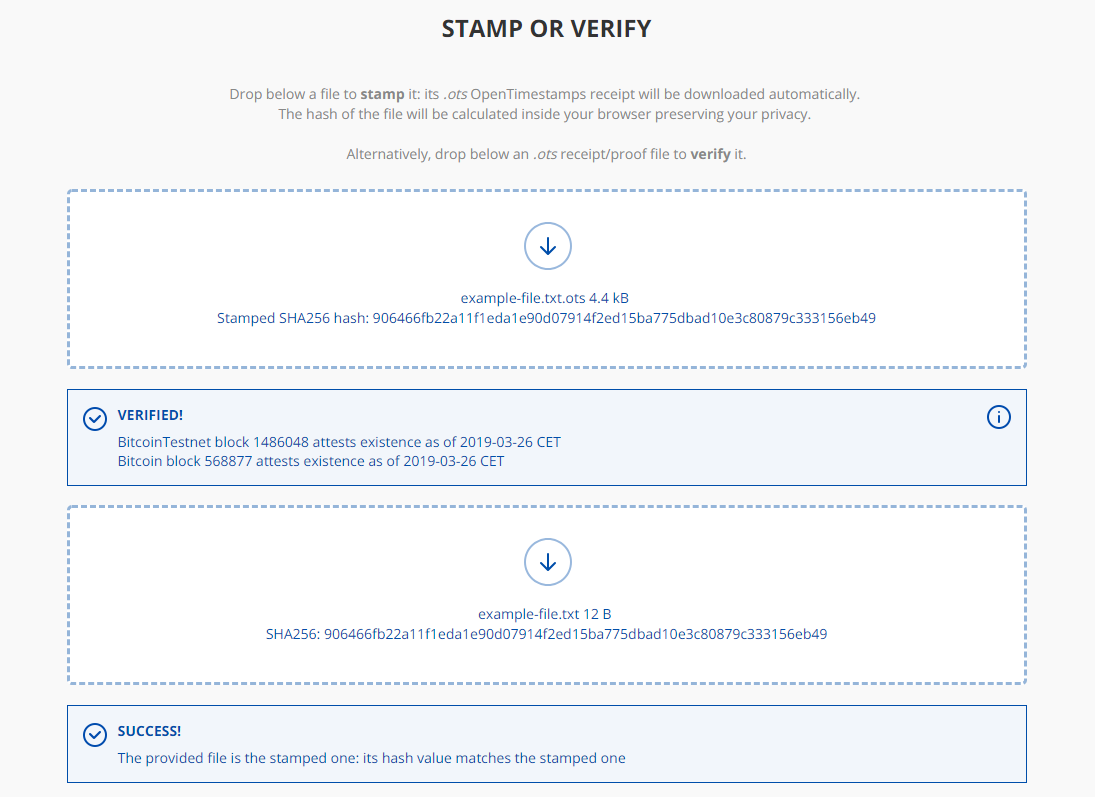
\includegraphics[width=0.85\linewidth]{Images/multivalidation.png}
         \caption{Multi-validation}
         
     \end{figure}
    \end{frame}
    
    \section{Conclusions}
     \begin{frame}{Conclusions and Future Work}
    \end{frame}
    
	
    \appendix
    \backupbegin
    \begin{frame}[t, allowframebreaks]
	\frametitle{References}
    	\setbeamertemplate{bibliography item}[text]
    	\bibliographystyle{plain}
		\nocite{*}
		\bibliography{biblio}
	\end{frame}
    
\backupend
\end{document}
  